\documentclass{sig-alternate}
\usepackage{multirow}
\usepackage[usenames, dvipsnames]{color}
\usepackage{colortbl}

\usepackage{picture}
\usepackage{wrapfig}
\usepackage{algorithm}
\usepackage{graphicx}
\usepackage{algorithmicx}
\usepackage{algpseudocode}
\renewcommand{\algorithmicrequire}{\textbf{Input:}}
\renewcommand{\algorithmicensure}{\textbf{Output:}} 
\newcommand{\lucas}[1]{\textcolor{red}{LUCAS: #1}} \newcommand{\tim}[1]{\textcolor{orange}{TIM: #1}}
\newcommand{\bill}[1]{\textcolor{blue}{BILL: #1}} 
\newcommand{\carter}[1]{\textcolor{cyan}{CARTER: #1}} 
\newcommand{\sei}[1]{\textcolor{RedViolet}{BILL/FORREST: #1}} 
\newcommand{\todo}[1]{\textcolor{Maroon}{TODO: #1}} 
%\newenvironment{changed}{\par}{\par}

%timm tricks
\newcommand{\bi}{\begin{itemize}[leftmargin=0.4cm]}
\newcommand{\ei}{\end{itemize}}
\newcommand{\be}{\begin{enumerate}}
\newcommand{\ee}{\end{enumerate}}
\newcommand{\tion}[1]{\S\ref{sect:#1}}
\newcommand{\fig}[1]{Figure~\ref{fig:#1}}
\newcommand{\eq}[1]{Equation~\ref{eq:#1}}
 

\usepackage[shortlabels]{enumitem} 
\usepackage{times}

\usepackage{cite}
\newcommand{\subparagraph}{}
\usepackage{url}
\def\baselinestretch{1}


\setlist{nosep}

\usepackage{colortbl}
 \usepackage[font={small}]{caption, subfig}
\setlength{\abovecaptionskip}{1ex}
 \setlength{\belowcaptionskip}{1ex}

 \setlength{\floatsep}{1ex}
 \setlength{\textfloatsep}{1ex}
\usepackage[compact,small]{titlesec}
\DeclareMathSizes{7}{7}{7}{7} 
\pagenumbering{arabic}
\setlength{\columnsep}{7mm}

\begin{document}

\conferenceinfo{FSE}{'15 Bergamo, Italy}
\title{Revisiting the Truisms of Software Engineering:\\ Does Phase Delay Dramatically Increases  Repair Time?}
\numberofauthors{3}
\author{
\alignauthor
Tim Menzies, \\Carter Pape\\
       \affaddr{CS, NcState, USA}\\
       tim.menzies@gmail.com,\\carterpape@gmail.com
\alignauthor
William Nichols,\\ Forrest Schull\\
\affaddr{SEI, CMU, USA}
wrn,fjshull@sei.cmu.edu
\alignauthor
Lucas \\Layman\\
       \affaddr{Fraunhofer Center,  USA}\\ 
       llayman@fc-md.umd.edu
} 


 
\maketitle
\begin{abstract}
Does
repair time increases dramatically
the longer a defect persists in a system?
This  is very widely belief that is used to justify 
radical changed to    traditional software development
 processes.

This paper shows that this belief is maintained
quite strongly in the industrial software engineering
community (but, in the academic community, somewhat less so).
Yet based on a sample of 
171 software projects from around the world from 
\bill{2005 to 2013}, we argue that this belief is mostly 
incorrect. Specifically: the median fix time for issues
is just a few minutes and this does not tend to increase
the longer the issue remains in the system. 

%This result raises the question: how did myths like phase delay survive so long  without  critical reassessment.  As a community, we need to reflect more on research practices and on how (and when) we reflect on the prominent hypotheses of our field.
\end{abstract}

% A category with the (minimum) three required fields
\vspace{1mm}
\noindent
{\bf Categories/Subject Descriptors:} 
D.2.8 [Software Engineering]: Process metrics.

 

\vspace{1mm}
\noindent
{\bf Keywords:} phase delay, time to fix, agile, waterfall.

\section{Introduction}
In 2013-2014, the time of 
eleven  million programmers~\cite{pettey14} and
half a trillion dollars~\cite{avram14} was spent on information technology.
Such a large and growing effort should be managed and optimized via  well-researched conclusions.  
It is standard practice
in other fields such as medicine,
to continually revisit old conclusions~\cite{prasad13}. Software engineering should do the same lest
ill-founded  exert an undue influence on how we build software.  

Accordingly, this paper revisits
the {\em phase delay effect}
i.e.,  the time required to resolve an issue in a software project increases dramatically 
the longer it remains in the system. 
Phase delay has long been
a    motivator for major changes to
SE practices. Basili \& Boehm comment that since the 1980s,  phase delay:
\begin{quote}
...has been a major driver in focusing
industrial software practice on thorough
requirements analysis and design,
on early verification and validation, and
on up-front prototyping and simulation
to avoid costly downstream fixes~\cite{boehm01}.
\end{quote}
Basili and Boehm are not alone in this assessment of the significance of the phase delay effect. Our surveys of industrial practitioners (shown in \S\ref{survey}) reveal the phase-delay effect to be
the single most strongly held belief amongst commercial SE engineers.
Previously~\cite{me08a}, we have constructed return-on-investement models
for a common practice amongst U.S. government contractors: 
independent verification \& validation. IVV has been criticized as
ineffective since IVV engineers, who many  unfamiliar with the details of the project, are required to pass judgement on the code.
Hence,  the IVV team may find the same or fewer bugs
as the developers,
On the other hand, IVV has been defended
as follows:  when the IVV team finds bugs earlier that the developers then, due to the phase delay effect, this saves the overall cost of the project. Note that the strength of this argument diminishes
if fixing later-phase issues is not significantly more expensive than fixing them earlier. 



% Also, as discussed later in this paper, concerns over phase delay were a major driver in the development of agile software processes.

In this paper, we investigate two hypotheses:

\bi
    \item $H_1$: The cost-to-fix of defects monotonically increases across phases.
    \item $H_2$: The cost-to-fix of defects monotonically increases as the phase delay increases.
\ei
The rest of the paper investigates these two hypotheses. First, we conduct a survey of practitioners and researchers to gauge their belief in the phase delay effect. Second, we  analyze 171 software  projects developed in the period \bill{2004 to 2014}.  To the best of our knowledge, this is the largest study on phase delay yet seen in the literature.

% The conclusions of this paper is that it is erroneous to believe in phase delay.
% When we looked for supporting evidence for that effect, we found that:
% \be 
% \item The evidence for that effect in the historical literature is very weak (to say the least);
% \item  In  a large sample of   contemporary software projects, there is no evidence for phase delay.
%  \ee
% The rest of this paper present evidence for the above two points. 



% The first point is  documented via  a literature survey and the second point is demonstrated
% via an analysis of  
 
 
The conclusions of this paper are two fold. First, the phase delay effect does not hold in the large body of software projects analyzed. Second, commonly-held beliefs, such as phase delay, must be periodically revisited empirically in order for researchers to provide accurate and up-to-date guidance for the practitioner community.

% the SE community needs to stop
% justifying changes to SE
% practices via the phase delay effect. Secondly,   myths like phase delay should not have lasted decades
% in the literature without  critical reassessment.  As a community, we need to reflect more on our
% research practices and on how (and when) we reflect and revisit the prominent hypotheses of our field.


\section{Motivation}
\subsection{Why Reassess Existing Triusms?}

Before exploring the commonly-held belief of the {\em phase delay effect}, we digress to discuss the merits of revisiting
old conclusions in software engineering.


Belief in general
principles of software
engineering are common to both research and practice. Processional societies assume such generalities exist when they offer
 lists of supposedly general ``best practices'' such as
the IEEE 1012 standard for software verification~\cite{1012}.  Endres \& Rombach's comment that 
\begin{quote}
Based on repeated and consistent observations, key lessons of these fields can now be formulated into rules or even laws, providing initial building blocks towards a theoretical foundation that is essential for further research, for teaching and for the practice of software development~\cite{endres03,rombach11}
\end{quote}
 Endres \& Rombach offer dozens of lessons of software engineering~\cite{rombach11}.
 Many other 
widely-cited researchers  do the same; e.g.
Glass~\cite{glass02}; Jones~\cite{jones07}; Boehm~\cite{boehm00b}.
Budgen \& Kitchenham seek to reorganize SE research using
general
conclusions drawn from a larger number of studies~\cite{kitch04,budgen09}.

Nevertheless, there are many empirical  findings that 
cast doubt on the existence of  ``key lessons  that can be formulated
as general laws of SE'':
\bi
\item
Turhan~\cite{me12d} lists 28 studies with contradictory conclusions
on the relation of OO measures to defects.  Those results
 directly  contradict some of the laws listed by 
Endres \& Rombach~\cite{endres03}.

\item
Ray et al.~\cite{ray2014lang} tested if   strongly typed languages
predict for better code quality. In  728 projects,
they found  only a modest benefit in strong typing
(and caution that that effect may actually be due to other  conflating factors).
\item
Fenton \& Neil~\cite{fenton00,fenton00b}   critique the truism that
``pre-release fault rates for software
are a predictor for post-release failures'' (as claimed by~\cite{dunsmore88},
amongst others). For the systems described in~\cite{fenton97}, they
show that software modules that were highly fault-prone
prior to release revealed very few faults after release.
\item
Meyer claims that   object-oriented (OO) encapsulation will
reduce error rates in software~\cite{Meyer1988}.  Yet empirical results suggest
that debugging an OO program is many times harder and
longer than debugging a standard procedural program~\cite{hatton98}.
\item A truism of visual programming is that ``visual
representations are inherently superior to mere textual representations''. A review by Menzies suggests that the available
evidence for this claim is hardly conclusive~\cite{me00v}. 
\item Numerous recent {\em local learning} results compare single models
learned from all available data to multiple models learned from clusters within the data~\cite{betten14,yang11,yang13,minku13,me12d,me11m,betta12,posnett11}.
A repeated result in those studies in that the local models generated the better effort
and defect predictions (better median results,
lower variance in the predictions).
 \item 
Other work studies  found dozens of single
models that performed worse that {\em committees of models}, all with different opinions,
that contribute to an {\em ensemble} prediction of software development effort~\cite{kocaguneli2012value,azhar13}.
\ei
%To be fair to the software engineering community,
Software engineering is not the only
field where practitioners hang on to persistent beliefs, even if the evidence
for those beliefs is not strong.
The medical profession applies  many practices based on studies
that have been disproved. For example,
a  recent article
in the Mayo Clinic Proceedings~\cite{prasad13} found  
146 medical practices based on studies 
in year $i$, but which were  reversed by subsequent trials within years $i+10$.
Even when the evidence for or against a treatment or intervention is clear, medical providers and patients may not accept it~\cite{aschwanden10}.
Aschwanden warns:
\begin{quote}
Cognitive biases - such as motivated reasoning (all of us want to believe that the things we do make a difference), base rate neglect (failing to pay attention to what happens in the absence of the intervention), and confirmation bias (the tendency to look for evidence that supports what you already know and to ignore the rest) - also influence how we process information~\cite{aschwanden15}.
\end{quote}

The cognitive issues that complicate medicine are also found in software engineering.
According to Passos et al.~\cite{passos11}, commercial developers
are all too willing to believe in general
truisms.
They  warn that developers
usually assume that the truisms they learn from a few past
projects are general to 
all their future projects:
\begin{quote}\label{q:pass}
...the past experiences were taken into account without 
much consideration for their context~\cite{passos11}.  
\end{quote}
The results of J{\o}rgensen \& Gruschke~\cite{jorgensen09} support the findings if Passos et al. They report that 
  supposed software engineering    ``experts'' rarely use lessons
  from past projects to improve their future reasoning~\cite{jorgensen09}. 
 They note that
when the experts
  fail to revise their beliefs, this leads to poor
 conclusions and software projects  (see examples in~\cite{jorgensen09}).
%% This leads to  detrimental
%% situations where groups or 
%% individuals working on the same project have conflicting beliefs, which they never debate
%or refine or unify.

In summary, just like medicine, our field suffers when
 software engineers do  revise old beliefs.  Therefore, it is important
 to regularly  reexamine    old beliefs.
 
\subsection{Why Study Phase Delay?}
\todo{\begin{itemize}
\item Given the Intro and Motivation, this section should focus on the influence of phase delay in software engineering milieux
\item Need to tone down the reliance on Beck. The important Beck point is that eliminating the cost-to-fix curve (resulting from phase delay) is one of the main goals of agile. His observations on new technologies are good too.
\item Need to cite other popular sources of this information, e.g., McConnell's "Ounce of Prevention" article~\cite{mcconnell01}.
\item Robert Glass's~\cite{glass02} book is very popular and contains an entry on this point
\item Google Scholar Citations for phase delay works Boehm88~\cite{boehm88} (673), Boehm \& Basili~\cite{boehm01} (761), 
\end{itemize}}

Due to its prominence in the field of software engineering,
this paper studies phase delay. As mentioned in the introduction, concerns about phase delay have
been used for decades to motivate major changes to software engineering practices. For example,
in 2000, Kent Beck used phase delay to motivate his call for ``extreme programming'' (a set of techniques
that evolved into contemporary agile and DevOps practices). Beck writes:
\begin{quote}
One of the universal assumptions of software engineering is that the cost of changing a program rises exponentially over time. I can remember sitting in a big linoleum-floored classroom as a college junior and seeing the professor draw on the board the curve found in \fig{curve1}.

The cost to fix a problem in a piece of software rises exponentially over time. A problem that might take a dollar to fix if you found it during requirements analysis might costs thousands to fix once the software is in production.

I resolved then and there that I would never let a problem get through to production. No sirree, I was going to catch problems as soon as possible. I would work out every possible problem in advance. I would review and crosscheck my code. No way was I going to cost my employer \$100,000.~\cite{beck00}
\end{quote}

\begin{figure}
 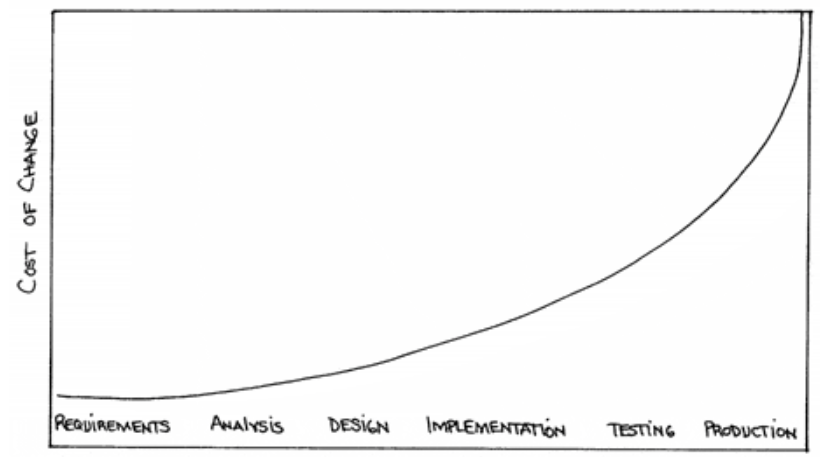
\includegraphics[width=3.3in]{beckB4.png}
 \caption{Projects exhibiting phase delay. From~\cite{beck00}.}\label{fig:curve1}
 \end{figure}
\begin{figure}
 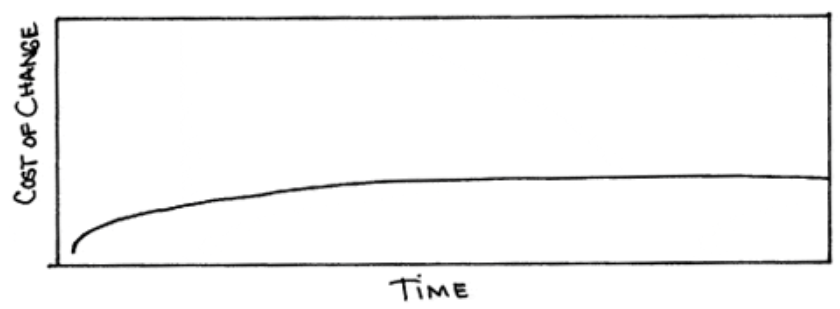
\includegraphics[width=3.3in]{beckAFTER.png}
 \caption{Projects without   phase delay. From~\cite{beck00}.}\label{fig:curve2}
\end{figure}

\begin{figure}[!t]
\scriptsize
\begin{center}
\begin{tabular}{l@{~}|l@{~}|r@{~}r@{~}|r@{~}l}
          &        & \multicolumn{2}{c|}{Time to}  &\\
          &        & \multicolumn{2}{c|}{resolve} &\\
Injection & Removal& initial & now & \multicolumn{2}{l}{Scale up w.r.t initial} \\\hline
Phase $i$&Phase $i$ & 1 & 1 & 1 & **\\
Phase $i$ &Phase $i+1$ & 1 & 2& 2 & **** \\
Phase $i$ &Phase $i+2$ & 1 & 4& 4 &******** \\
Phase $i$ &Phase $i+3$ & 1 & 8 & 8 & ****************  
  \end{tabular}\end{center}
 \caption{Projects data consistent with
 the phase delay effect of \fig{curve1}.}\label{fig:curve1a}
\end{figure}

\begin{figure}[!t]
\scriptsize
\begin{center}
\begin{tabular}{l@{~}|l@{~}|r@{~}r@{~}|r@{~}l}
          &        & \multicolumn{2}{c|}{Time to}  &\\
          &        & \multicolumn{2}{c|}{resolve} &\\
Injection & Removal& initial & now & \multicolumn{2}{l}{Scale up w.r.t initial} \\\hline
Phase $i$&Phase $i$ & 1 & 1 & 1 & ** \\
Phase $i$ &Phase $i+1$ & 1 & 2& 2 & **** \\
Phase $i$ &Phase $i+2$ & 1 & 2& 2 & **** \\
Phase $i$ &Phase $i+3$ & 1 & 2 & 2 & **** \\
 Phase $i$  &Phase $i+4$ &1 & 2& 2 &**** 
  \end{tabular}\end{center}
 \caption{Projects data consistent with
 the phase delay effect of \fig{curve2}.}\label{fig:curve2a}
\end{figure}
 
Beck speculated that there might be another kind of project, shown in \fig{curve2},
that does no exhibit phase delay. In this next quote, Beck clearly states
the importance of avoiding phase delay (in fact, for Beck, it is {\em the} major
motivation for his work):
\begin{quote}
This (\fig{curve2}) is one of the premises of (agile). It is the technical premise of (agile). If the cost of change rose slowly over time, you would act completely differently from how you do under the assumption that costs rise exponentially. You would make big decisions as late in the process as possible, to defer the cost of making the decisions and to have the greatest possible chance that they would be right. You would only implement what you had to, in hopes that the needs you anticipate for tomorrow wouldn't come true. You would introduce elements to the design only as they simplified existing code or made writing the next bit of code simpler.~\cite{beck00}
\end{quote}
Beck makes one other comment that is relevant to this paper: 
\begin{quote}
The software development community has spent enormous resources in recent decades trying to reduce the cost of change-better languages, better database technology, better programming practices, better environments and tools, new notations.

What would we do if all that investment paid off? What if all that work on languages and databases and whatnot actually got somewhere? What if the cost of change didn't rise exponentially over time?~\cite{beck00}
\end{quote}
The results of this paper are that, in our sample of hundreds of projects, there is no evidence for phase delay.
This result is   consistent with Beck being correct: all that work on    languages and databases
have paid off and, hence, modern software projects do not suffer from the  phase delay effect.  

XXX clumsy link here
That said, where our results
diverge from Beck is that we have observed this lack of phase delay in  projects that are not agile. Those
projects are described below.

\section{Related Work}
 

The first data on the cost to fix defects as a function of lifecycle phase date back to large systems in the late 70s from IBM~\cite{Fagan76}, TRW~\cite{Boehm76}, GTE~\cite{Daly77}, and Bell Labs~\cite{Stephenson76} (Figure~\ref{fig:cost-to-fix}). These studies suggest that the cost (in terms of effort) to find and fix an error monotonically increases with lifecycle phase. For large projects, the ratio of cost-to-fix in the requirements phase to cost-to-fix in operation is on the order of 1:100. Furthermore, cost function is superlinear, with the greatest rates of increase in the acceptance testing and operations phases.

\begin{figure}[!ht]
 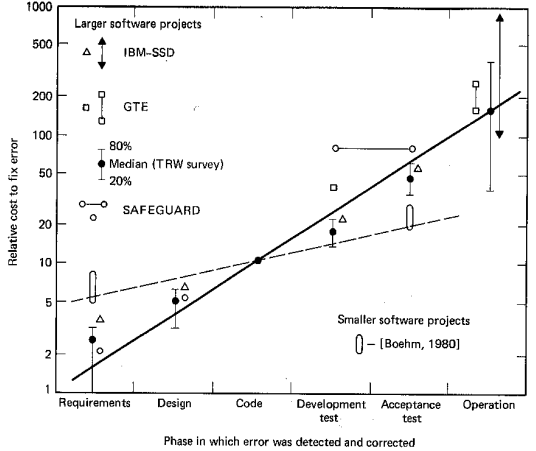
\includegraphics[width=3.3in]{boehm_cost-to-fix.png}
 \caption{Historical cost-to-fix curve. From~\cite{Boehm81}.}\label{fig:cost-to-fix}
 \end{figure}
 
In the 40 years since these initial studies, few studies have been published on the cost-to-fix curve as a function of lifecycle phase. Boehm~\cite{Boehm80} provides data suggesting that the cost-to-fix curve for small projects (from two student projects of 2000 deliverable source instructions) is flatter than for large projects (the dashed line of Figure~\ref{fig:cost-to-fix}). Shull et al.~\cite{Shull02} conducted a literature survey and held a series of e-workshops with industry experts on fighting defects. Workshop participants from Toshiba and IBM reported cost-to-fix ratios of 1:137 and 1:117 for large projects respectively~\cite{Shull02} -- the raw data points are not provided. One notable example to the traditional cost-to-fix curve is the CCPDS-R described by Royce~\cite{Royce98}: a million-line, safety-critical missile defense system (Figure~\ref{fig:royce}). In this project, design changes (including architecture changes) required approximately twice the effort of implementation and test changes, and the cost-to-fix in implementation and test phases increased slowly. Boehm~\cite{Boehm10} attributes this success to the CCPDS-R development process, which focused on removing architecture risk early in the development lifecycle.

\begin{figure}[!ht]
 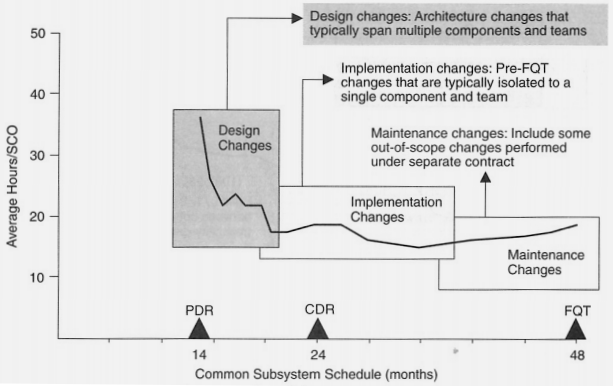
\includegraphics[width=3.3in]{Royce98.png}
 \caption{Exception to the rule - CCPDS-R case study cost-to-fix curve. From~\cite{Royce98}.}\label{fig:royce}
 \end{figure}
 
As discussed is \S\ref{sec:why-study}, one goal of agile methods is to flatten the cost-to-change curve~\cite{beck00}. Relatively little empirical data exists on this point. Clutterbuck et al.~\cite{Clutterbuck09} studied 5-month effort by a small-to-medium enterprise team developing a 71KLOEC web interface to a database application to implement 18 change requests (Figure~\ref{fig:clutterbuck}). Note that these were for new and changed user requirements, not defects. Clutterbuck et al. found the cost of change to be relatively flat until the later phases, with much of the effort spent in analysis of the change requests~\cite{Clutterbuck09}. Elssamadisy and Schalliol~\cite{Elssamadisy02} anecdotally report on the growing, high cost of rework in a 50 person, three-year, 500KLOEC Extreme Programming project as the project grew in size and complexity.

\begin{figure}[!ht]
 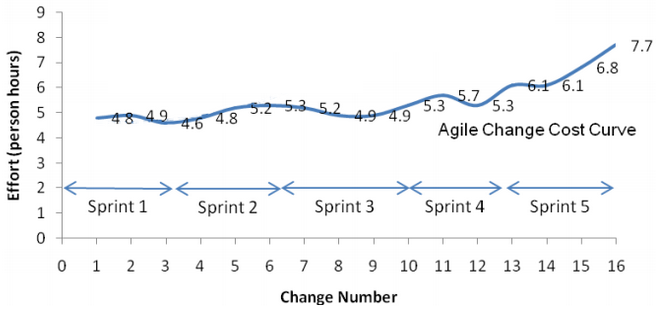
\includegraphics[width=3.3in]{clutterbuck.png}
 \caption{Cost of change from an agile case study. From~\cite{Clutterbuck09}.}\label{fig:clutterbuck}
 \end{figure}
 
 We note that previous work focuses on cost-to-fix as a function of lifecycle phase irrespective of when the defect was injected, that is, previous work analyzes the cost to fix a defect found in test regardless of whether that defect was a requirements error or a coding mistake. To our knowledge, our research represents the first large-scale study of phase delay.

\section{A Survey on Phase Delay and Cost-to-fix Belief}
\label{survey}






Our survey collected data on software engineers' views of commonly held software engineering ``laws''.
One of the laws questioned relates directly to phase delay: ``Requirements errors are the most expensive to fix when found during production but the cheapest to fix early in development'' (from Glass~\cite{glass02} p.71 who references Boehm \& Basili~\cite{boehm01}). We abbreviate this law as RqtsErr. 

The survey was conducted in two phases using Amazon's Mechanical Turk. The first phase was conducted only with professional software engineers solicited through the Mechanical Turk\footnote{Professional software engineers were required to complete a pretest to verify their status as a professional or open source software developer and to confirm their knowledge of basic software engineering terminology and technology.}, and the second survey was conducted Program Committee members of the ESEC/FSE and ICSE conferences solicited via email.

The respondents answered the following questions for the laws they were presented: \newline
\textbf{Agreement:} ``Based on your experience, do you agree that the statement above is correct?'' A Likert scale captured the agreement score from Strongly Disagree to Strongly Agree. A text box was provided to explain the answer. \newline
\textbf{Applicability:} ``To the extent that you believe it, how widely do you think it applies among software development contexts?'' The possible answers were presented as a scale from -1 to 5:
\begin{itemize}
\item I don't know (-1)
\item This law does not apply at all (0)
\item Applies in a very narrow range of projects  (1)
\item Rarely applies (2)
\item Occasionally applies (3)
\item Very frequently applies (4)
\item Always applies (5)
\end{itemize}
Respondents were required to explain the applicability score in a text box.

Participants were presented with the RqtsErr law and others drawn from \cite{glass02} and \cite{endres03}. The PC member survey contained an additional question on ``In general, the longer errors are in the system (requirements errors, design errors, coding errors, etc.), the more expensive they are to fix'' (PhaseDelay for short). Responses were recorded using the Agreement question Likert scale. 

Summary statistics for the agreement and applicability scores for the RqtsErr and PhaseDelay laws are presented in Figure~\ref{fig:survey_results}. Responses whose Applicability response was ''I don't know'' are ommitted from analysis.


\begin{figure}[!ht] 
\scriptsize
\begin{center}
\subcaption{Practitioner survey}
\begin{tabular}{l|c|c|c|c|c}
Law & N & \multicolumn{2}{c}{agreement} & \multicolumn{2}{c}{applicability} \\ 
 & & $\bar{x}$ & $\tilde{x}$ & $\bar{x}$ & $\tilde{x}$ \\
\hline 
\textbf{Rqts errors are most expensive...} & 16 & 4.6 & 5 & 4.2 & 4 \\ 
Process maturity improves output & 17 & 4.4 & 4 & 3.9 & 4 \\ 
Most time is spent removing errors & 16 & 4.1 & 4 & 3.9 & 4 \\ 
Missing reqts are hardest to fix & 17 & 4.1 & 4 & 4.0 & 4 \\
Reuse increases prod. and qual. & 16 & 3.9 & 4 & 3.8 & 4 \\
OO-programming reduces errors & 13 & 3.9 & 4 & 3.5 & 4 \\
80-20 rule (defects to modules) & 12 & 3.8 & 4 & 4.0 & 4 \\
Adding manpower to a late project & 15 & 3.7 & 4 & 3.7 & 4 \\
Inspections can remove 90\% of defects & 18 & 3.3 & 4 & 3.5 & 4 \\
Smaller changes have higher error density & 14 & 2.8 & 3 & 3.4 & 3.5 \\
A developer is unsuited to test own code & 17 & 2.6 & 3 & 3.5 & 4
\end{tabular} 
\bigskip
\subcaption{Researcher survey}
\begin{tabular}{l|c|c|c|c|c}
Law & N & \multicolumn{2}{c}{agreement} & \multicolumn{2}{c}{applicability} \\ 
 & & $\bar{x}$ & $\tilde{x}$ & $\bar{x}$ & $\tilde{x}$ \\
\hline 
Process maturity improves output & 4 & 4.0 & 4 & 4.0 & 4 \\
\textbf{Rqts errors are most expensive...} & 30 & 3.8 & 4 & 3.8 & 4   \\ 
80-20 rule (defects to modules) & 6 & 3.7 & 4 & 3.5 & 4 \\
\textbf{PhaseDelay} & 30 & 3.6 & 4 & -- & --  \\ 
Missing reqts are hardest to fix & 7 & 3.6 & 4 & 3.7 & 4 \\
Adding manpower to a late project & 4 & 3.5 & 4 & 3.5 & 4 \\
Inspections can remove 90\% of defects & 7 & 3.4 & 4 & 3.6 & 3 \\
Reuse increases prod. and qual. & 6 & 3.3 & 4 & 3.0 & 4 \\
OO-programming reduces errors & 6 & 3.2 & 4 & 2.7 & 3 \\
Most time is spent removing errors & 6 & 2.8 & 3 & 3.2 & 4 \\ 
Smaller changes have higher error density & 4 & 2.8 & 3 & 4.0 & 4 \\
A developer is unsuited to test own code & 7 & 2.1 & 2 & 2.4 & 3
\end{tabular} 

\end{center}
\caption{Agreement and applicability of software engineering axioms.}
\label{fig:survey_results}
\end{figure}

While the practitioners strongly believed in the law, researchers were less firm. In the free response texts, most participants agreed that addressing errors late may mean system redesign unless the system and the affected requirement are simple/trivial. Further, any changes to the production system have additional complexity (compared to changes while system in development) due to users, data existence, and architecture dependencies. The researchers who disagreed with the law generally asserted that requirements change can be expensive, but that depends on the process used (e.g., agile vs. waterfall) and the adaptability of the system architecture.

Overall, the RqtsErr law was the most agreed upon and most applicable law of 11 surveyed amongst practitioners, and the second most agreed upon law amongst researchers. The survey results seem to confirm that the notion that phase delay escalates cost-to-fix is a widely-held belief in software engineering.





%\section{carterCharts}

%anything

 
\begin{figure*}[!t]
\begin{center}
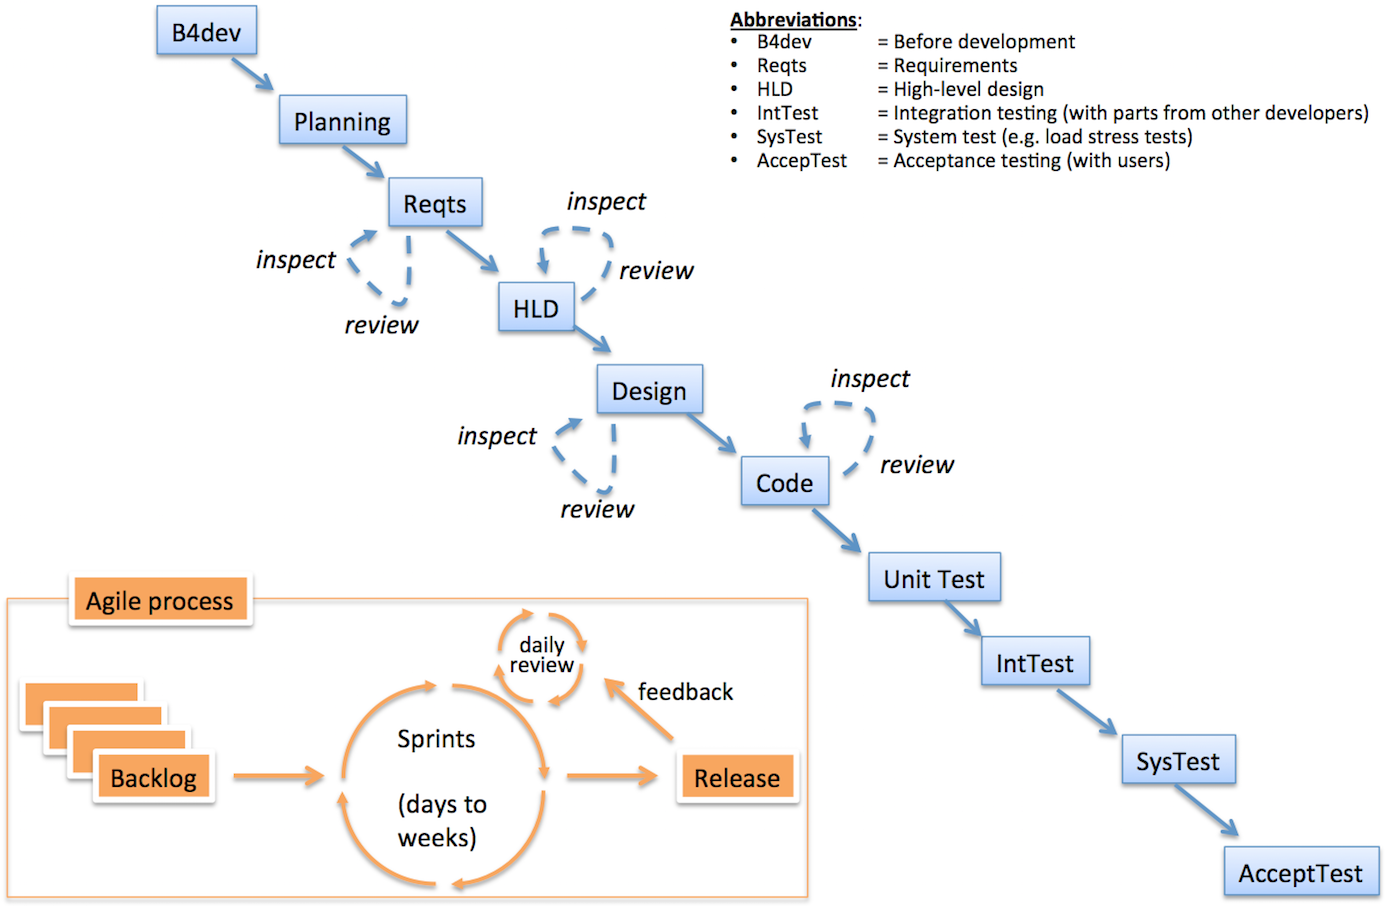
\includegraphics[width=6in]{waterfall3.png}
\end{center}
\caption{Different approaches to software development:  waterfall and agile (bottom left).}
\label{fig:waterfall}
\end{figure*}

\section{Data Collection}


Before presenting our analysis of phase delay in software projects, we define our terms, provide an overview of TSP and the sample projects, and describe the data collection process.

\subsection{Definitions}
A \emph{defect} is any change to a product, after its construction, that is necessary to make the product correct.  A typographical error found in review is a defect. If that same defect is discovered while writing the code but before review, it is not considered to be a defect. 

The \emph{cost-to-fix} can be computed in two ways. The first is a direct measure of the actual work time spent in correcting the defect in the product. Direct measurement enables analysis of the variability the cost-to-fix among a category of defects. The second approach measures the total time spent in a defect removal phase and divides by the total defects removed. This provides an average cost-to-fix including overhead of that activity. For example, using method two, a code inspection may require an hour of effort to remove three defects for a 3 defects per hour or to invert the ratio, 1/3 hours per defect. Most of the time, however, is spent locating the defects not actually fixing them. we use the second approach in our analysis.


\subsection{Overview of the Team Software Process}
To empirically test for the phase delay effect, we examined 171 software projects conducted between 2005 and 2014. These projects took place at organizations in many countries and were conducted using  the Team Software Process (TSP$\textsuperscript{SM}$), a software project management approach developed at the Software Engineering Institute (SEI) at Carnegie Mellon University~\cite{tsp00}. TSP is an extension of the Personal Software Process (PSP$\textsuperscript{SM}$) developed at the SEI by Watts Humphrey ~\cite{tsp00}. The data from these TSP projects were collected and stored in the Software Engineering Measured Process Repository (SEMPR) at the SEI. The Software Engineering Institute (SEI) at Carnegie Mellon University explores methods for software process improvement.
 



TSP has guiding principles; the following are relevant to this study:
\begin{itemize}
\item  Sound engineering work does not happen by accident. It must be planned.
\item  Performance of the plans requires realistic commitments of the resources needed to perform the work.
\item  The planned work should frequently be compared to  results to assure plans remain relevant.
\item  People performing the work should be responsible for planning and tracking the work.
\end{itemize}

TSP helps developers by providing a set of measures that can be applied to managing tasks, quality, and schedule. Planning begins by quantifying goals, defining work practices, and estimating size and effort. Developers then use this information to make a detailed short term plan. As the developers perform project work, they use a tool such as the Process Dashboard to collect their time, effort, size, and schedule data. Every week, the team reviews their data to evaluate status, identify actual rates, determine if project goals for schedule, cost, and quality are being met. The team then uses this information to make necessary plan corrections. At the end of the project the coach and team perform a quantitative project post mortem.

Common features of TSP projects include {\em planning}, {\em personal reviews}, {\em peer inspections}, and {\em coaching}.
A TSP {\em coach} helps the team to plan and analyze performance. The coach is the only role authorized to submit project data to the SEI.
Before reviewing data with the teams, therefore before submission, these coaches check the data for obvious errors.

{\em Planning} follows the technique taught in the PSP$\textsuperscript{SM}$. Developers estimate the size of work products and convert this to a total effort using historical rates. Time in specific tasks come from the  process phases and historical percent time in phase distributions. Defects are estimated using historical phase injection rates and phase removal yields. Coaches help the developers to compare estimates against actual results. In this way, developers acquire a more realistic understanding of their work behavior, performance, and schedule status.

{\em Personal review} is a technique taken from the PSP and its use in TSP is unique.  Developers follow a systematic process to remove defects by  examining their own work products using a checklist built from their personal defect profile. This personal review occurs after some product or part of a product is considered to be constructed and before peer reviews or test. 

%PSPSM teaches developers howto continually make and review their personnel estimates
%about their day-to-day tasks, then compare those estimates against the actual development effort.
%In this way, developers can acquire a more realistic understanding of their work behaviour.
  
 
{\em Peer inspection} is a  technique in
traditional software engineering and is often called peer review.
 Basili and Boehm   commented in 2001~\cite{boehm01} 
that peer reviews can catch over half the defects introduced into a system.
Peer inspection can be conducted on any artifact generated anywhere in the software
lifecycle and can quickly be adapted to new kinds of artifacts. TSP peer reviews follow the Fagan style in which the reviewer uses a checklist composed of common team defects prior to a review team meeting. 


\begin{figure}[!t]  
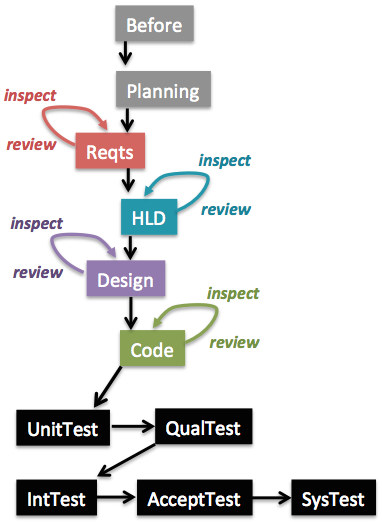
\includegraphics[width=4in]{img/waterfall-v3.png}  
\caption{Different approaches to software development:  waterfall and agile (bottom left).}
\label{fig:waterfall}
\end{figure}


\subsection{Projects in the Sample}
Since shortly before the year 2000, the SEI has been teaching and coaching TSP teams. One of the authors (Nichols) has been been mentoring software development teams and coaches around the world as they deploy TSP within their organizations since 2006.  The  most recent completions were in 2014.
The projects were mostly small to medium, with a median duration of 46 days and a maximum duration of 90 days in major increments. 
Several projects extended for multiple incremental development cycles. 
Median team size was 7 people, with a maximum of 40. 

Many of the projects were e-commerce web portals or banking systems in the US, South Africa, and Mexico. 
There were  some  medical device projects in  the US, France, Japan, and Germany as well  as a commercial computer-aided design systems, and embedded systems. 

An anonymized version of that data is available in the PROMISE repository\footnote{http://openscience.us/repo}  and,
for confidentiality restrictions, we cannot offer 
further details on these projects.



\subsection{Data Collection Process}
\label{sec:data-collection}

Organizations using TSP agree to provide their project data to the SEI for use in research. In return the SEI agrees    that  data must not be traceable to its source. The data is collected at major project events; launch, interim checkpoints, and at project completion. Data includes project and site  characteristic summaries, surveys of team members, launch presentations, launch outbriefs, and baseline plans, final data from the project, and the project post mortem report.  In practice, this data requirement has only been enforced for the purposes of certifying and reauthorizing TSP coaches who must submit data to maintain their authorization. Coaches are certified by demonstrating competent use of the TSP process with the artifacts and data not by the actual project results.  Of the data submitted, only the data recorded using the Process Dashboard tool has been collected and aggregated for this research. 

To use this data for research and benchmarking,  Nichols first collected the Process Dashboard data from the submission repository then used a tool built by the Process Dashboard developer, David Tuma, 
to gather the project data into a database. Nichols and his colleague Yasutaka Shirai then extracted data into views suitable for analysis. The key views include a project results summary, effort logs, task logs, and defect logs. The data has not yet undergone additional screening. A summary of the data quality issues was reported in a previous work ~\cite{shirai14} (that summary is discussed further in our {\em Validity} section, below).

The tool collected process information about those tasks and defects that we analyze in this work. 
That task data include  work start time, work end time, delta
work time, and interruption time. Software engineers are often
interrupted by meetings, requests for technical help, reporting, and
so forth. These events are recorded, in minutes, as interruption
time. 

 Defect logs include the time and date a defect was discovered, the phase in which that defect was injected, the phase in which it was removed, the time (in minutes) required to find and fix the defect, and the categorical type.

The defect types in the most common defect type standard  in the the SEI TSP data are follows:
\begin{itemize}
\item Environment: design, compile, test, or other support system problems
\item Interface: procedure calls and reference, I/O, user format
\item Data: structure, content
\item Documentation: comments, messages
\item Syntax: spelling, punctuation typos, instruction formats
\item Function: logic, pointers, loops, recursion, computation, function defects  
\item Checking: error messages, inadequate checks
\item Build: change management, library, version control
\item Assignment: package
declaration, duplicate names, scope, limits
\item System: configuration, timing, memory
\end{itemize}


As of November 2014, the SEI TSP database contained data from 212
TSP projects. The projects completed between July 2006 and
November 2014; they included 47 organizations and 843 people. 
The database fact tables
contain 268,726 time logs, 
154,238 task logs,
 47,376 defect logs, 
and 26,534 size logs. 
After selecting defects from the data log and joining the data to the time log table  171 of these projects remained. The excluded projects had no or too few defects to use in this analysis.
 
In this paper, when we report ``time to resolve an
issue,'' we show the difference between the start and end times
of a work session, with any interruption time subtracted (the
difference in times, minus the interruptions). 


%That said, certain semantic features of the SEI TSP data should be noted.
%Firstly, in the current TSP collection tool, 
%fix times are only the developer time for the developer walking through the phases of \fig{waterfall}.
%We are currently tracking the fix time for post-release issues (e.g. those raised during  acceptance test and %later
%product life cycle). So far, in that post-release data,  we have not detected
%a dramatic phase escalation effect (but at this time, we have nothing definitive comment on that matter).%
%
%\bill{somewhere you have one note on \underline{find} and fix times.  for this paper, we need just fix times. %but is there
%anything we need to fret about re \underline{find} times?}
 
 

\subsection{Project Phases}
This paper studies the impact of phase delay on the time required to resolve issues.
The logical phases used in this paper are shown in \fig{waterfall}. Although the representation suggests a waterfall, the phases represent the primary stages through which requirements are developed into working and tested code. That is, all requirements must be stated in some way, implemented in code, integrated, and tested. All real implementations of any size follow a spiral approach with many team performing the work in iterative and/or incremental development cycles.  Within a project increment, multiple features or components may be developed and incremented. TSP is compatible with agile and encourages iterative and incremental development. Nonetheless, the specific strategy and cycle duration is a project decision. TSP does, however, strongly encourage 1) constructing units of sufficient size that measurement is practicable, and 2) separating the construction from appraisal and test activities. This effectively highlights the separation of construction from rework activities and aids the apportionment of defects to those found in appraisal activities (reviews and inspections) and those found through failure (test). The distinct construction activities (requirements, high and detailed design, and code) were chosen to help teams analyze the effectiveness and efficiency of their practices through analysis of the defect phase origin, type, fix effort, and phase of discovery. 

Note that, in that Figure~\ref{fig:waterfall}:
\bi 
\item
Several  phases in which product is created have sub-phases of {\em review} and {\em inspect} to remove defects. TSP uses review, a sub-phase in which individuals perform personal reviews of their work products prior to the peer review, which TSP calls the inspection.
\item Testing is divided into several stages. Developers perform unit test prior to code complete.  After code complete a standard phase is the integration, which combines program units into workable system ready for system test. Integration,  system test, and acceptance test are often performed by a separate group. 
\ei
For these TSP projects, the principles followed are: 
\bi 
%\item Defects should be found before test, that is, test defects should be infrequent.
\item A product should be inspected before used in a subsequent construction phase to minimize  unnecessary rework.
\item To minimize unnecessary rework, a product should be reviewed and inspected prior to use in a subsequent construction phase.
\item A personal review should remove the most common defects before being given to peers for the inspection.
\item Because different categories of test will find different types of defect, and follow in a natural sequence, the tests should be measured separately
\ei 
In summary, the TSP process and measurement have been specifically designed to aid the analysis of defects for use in process improvement. The data are, therefore, uniquely suitable for an analysis of the phase delay effect. 
\subsection{Distinguishing Project Characteristics}
Modern development processes include the core engineering practices of estimation, planning, configuration control, requirements, design, code development, and test. Agile methods address  not only these core practices but also address team organization, individual and team commitments, test and build automation, and implementing iterative and incremental development. TSP uses additional practices associated with high performance ~\cite{jones10} including; project tracking and control, specialization of team members, inspections, static analysis, documentation and training, and reuse. Although the teams in this sample use many typical agile practices, they are also using additional practices. 










\section{Analysis of Phase Delay in 171 TSP Projects}

\todo{
\bi
    \item What is the cost-to-fix curve in TSP data? Check against H1 and compare to past literature.
    \item What is the effect of phase delay? Check against H2.
\ei
}


\subsection{TSP Project Cost-to-fix curve}

The distribution of defects found and fixed per phase is shown in Figure~\ref{fig:fix-phase-dist}. A high percentage of defects were found and fixed in the early phases, i.e., requirements, high level design, and design reviews and inspections. \todo{How does this compare evidence from other sources?}

The median time to fix a defect in each phase is shown in \fig{fix-time-per-phase}. \todo{Overlay median on Boehm's chart \fig{cost-to-fix}. How does it compare?}




\begin{figure}[!ht]
\begin{center}
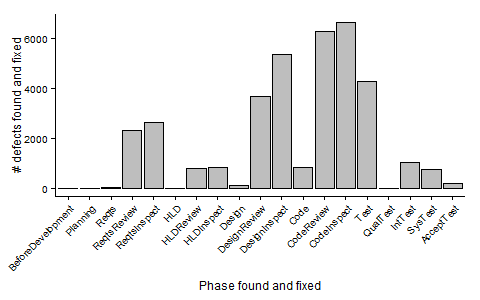
\includegraphics[width=3.3in]{fix-phase-dist.png}
\end{center}
\caption{Distribution of defects found and fixed by phase.}
\label{fig:fix-phase-dist}
\end{figure}



\begin{figure}[!ht]
\begin{center}
\begin{tabular}{r|rrr|l}
  Sample&\multicolumn{3}{c|}{Percentiles}\\ 
size & 25th & 50th & 75th & Phase removed \\
\hline
120 & 3 & 3 & 18 & ReqtsInspect.dat \\
126 & 3 & 3 & 20 & ReqtsReview.dat \\
70 & 2 & 2 & 10 & HLDInspect.dat \\
 55 &    2 &    1&    7&HLDReview.dat \\

278&    7&    7&   33&DesignInspect.dat \\
233&    6&    6&   25&DesignReview.dat \\

315&    8&    7&   34&CodeInspect.dat \\ 
282&    7&    7&   32&CodeReview.dat\\ 

425&   11&   10&   54&UnitTest.dat \\ 
226&    7&    6&   46&IntTest.dat \\ 
194&    7&    6&   52&SysTest.dat\\ 
 88&    4&    3&   38&AcceptTest.dat\\
\end{tabular}
\end{center}
\caption{Median fix time per phase}
\label{fig:fix-time-per-phase}
\end{figure}

We reject $H_1$.

\subsection{Phase delay analysis}
\todo{
\bi
    \item What can we say about \fig{raw}
    \item What can we say about \fig{scale}
    \item What is the difference between \fig{raw} and \fig{scale}
\ei
}

In the TSP data, there is a weak correlation (Kendall's $\tau = 0.19, p < 0.01, 95\% CI$) between a defect's cost-to-fix (minutes of effort) and the defects phase delay (phase removed - phase injected). The correlations were also calculated for each phase, e.g., does the phase delay of defects found in Test correlate with the defect's cost-to-fix (Table~\ref{tab:phase_corr}). 

We reject $H_2$.




\begin{figure*}[!t] 
 \renewcommand{\baselinestretch}{0.7}
 \scriptsize
\begin{center}
\begin{tabular}{r|rrr|ll|rl}
  Sample&\multicolumn{3}{c|}{Percentiles}\\ 
size & 25th & 50th & 75th & Phase injected & Phase removed & \multicolumn{2}{l}{Scale up w.r.t. to first phase}\\\hline
\\
  29 &     1 &     3 &    12 & Before & CodeInspect  & 1.00  &  **  \\
  26 &     1 &     4 &     6 & Before & CodeReview  & 1.33  &  ***  \\
  73 &     5 &    13 &    59 & Before & UnitTest  & 4.33  &  *********  \\
  36 &     7 &    24 &    54 & Before & IntTest  & 8.00  &  ****************  \\
  34 &     8 &    28 &    56 & Before & SysTest  & 9.33  &  *******************  \\\hline
\\
128 &     2 &     6 &    15 & Reqts & ReqtsInspect  & 1.00  &  **  \\
132 &     2 &     5 &    12 & Reqts & ReqtsReview  & 0.83  &  **  \\
 28 &     3 &    13 &    29 & Reqts & DesignInspect  & 2.16  &  *****  \\
 22 &     6 &    14 &    31 & Reqts & DesignReview  & 2.33  &  *****  \\\hline
\\
272 &     6 &    14 &    30 & Design & DesignInspect  & 1.00  &  **  \\
 32 &     1 &     4 &    13 & Design & DesignInspection  & 0.28  &  *  \\
240 &     4 &    11 &    22 & Design & DesignReview  & 0.78  &  **  \\
110 &     3 &    11 &    23 & Design & CodeInspect  & 0.78  &  **  \\
 91 &     3 &     7 &    18 & Design & CodeReview  & 0.50  &  *  \\
323 &     8 &    21 &    45 & Design & UnitTest  & 1.50  &  ***  \\
 56 &     7 &    20 &    41 & Design & IntTest  & 1.42  &  ***  \\
 69 &     9 &    27 &    53 & Design & SysTest  & 1.92  &  ****  \\\hline
\\
310 &     6 &    15 &    31 & Code & CodeInspect  & 1.00  &  **  \\
285 &     5 &    14 &    29 & Code & CodeReview  & 0.93  &  **  \\
287 &     7 &    17 &    44 & Code & UnitTest  & 1.13  &  ***  \\
180 &     7 &    20 &    45 & Code & IntTest  & 1.33  &  ***  \\
137 &     6 &    15 &    35 & Code & SysTest  & 1.00  &  **  \\
 37 &     1 &    11 &    27 & Code & AcceptTest  & 0.73  &  **  \\

 \end{tabular}
\end{center}
\caption{Distribution of fix times seen in SEI TSP data.}
\label{fig:raw}
\end{figure*}





 
 \begin{figure}[!t]
\renewcommand{\baselinestretch}{0.7}
\scriptsize
\begin{center}
\begin{tabular}{l@{~~}|l@{~}|r@{~}|r@{~}r@{~}|r@{~}l}
           \multicolumn{2}{c}{~}                 &  &\multicolumn{2}{c|}{median}\\
  Injection&   Removal& $n$ & initial & now & \multicolumn{2}{l}{Scale up, w.r.t. initial}
\\\hline

BeforeDevelopment&Code.dat&57&1&\rule{2mm}{2mm} \\
BeforeDevelopment&CodeInspect.dat&72&0.3&\rule{0mm}{2mm} \\
BeforeDevelopment&Test.dat&165&1.1&\rule{2mm}{2mm} \\
BeforeDevelopment&IntTest.dat&50&1.3&\rule{2mm}{2mm} \\
BeforeDevelopment&SysTest.dat&42&1.8&\rule{2mm}{2mm} \\
\\\hline

Planning&Planning.dat&66&1&\rule{2mm}{2mm} \\
Planning&ReqtsReview.dat&41&0.8&\rule{0mm}{2mm} \\
\\\hline

Reqts&Reqts.dat&23&1&\rule{2mm}{2mm} \\
Reqts&ReqtsReview.dat&245&13&\rule{26mm}{2mm} \\
Reqts&ReqtsInspect.dat&289&16&\rule{32mm}{2mm} \\
Reqts&Design.dat&32&21&\rule{42mm}{2mm} \\
Reqts&DesignInspect.dat&49&7&\rule{14mm}{2mm} \\
\\\hline
 

HLD&HLDReview.dat&94&1&\rule{2mm}{2mm} \\
HLD&HLDInspect.dat&133&1.6&\rule{2mm}{2mm} \\
HLD&Design.dat&33&1&\rule{2mm}{2mm} \\
\\\hline

Design&Design.dat&37&1&\rule{2mm}{2mm} \\
Design&DesignInspect.dat&455&6&\rule{12mm}{2mm} \\
Design&Code.dat&218&3.5&\rule{6mm}{2mm} \\
Design&CodeInspect.dat&166&2.7&\rule{4mm}{2mm} \\
Design&Test.dat&542&7.7&\rule{14mm}{2mm} \\
Design&IntTest.dat&67&3.7&\rule{6mm}{2mm} \\
Design&SysTest.dat&92&6.3&\rule{12mm}{2mm} \\
\\\hline

DesignInspect&DesignInspect.dat&53&1&\rule{2mm}{2mm} \\
DesignInspect&Code.dat&38&0.75&\rule{0mm}{2mm} \\
\\\hline

Code&Code.dat&126&1&\rule{2mm}{2mm} \\
Code&CodeInspect.dat&459&2&\rule{4mm}{2mm} \\
Code&Test.dat&461&2.16667&\rule{4mm}{2mm} \\
Code&IntTest.dat&348&2.16667&\rule{4mm}{2mm} \\
Code&SysTest.dat&230&1.5&\rule{2mm}{2mm} \\
Code&AcceptTest.dat&71&0.916667&\rule{0mm}{2mm} \\
\\\hline

CodeInspect&CodeInspect.dat&64&1&\rule{2mm}{2mm} \\
CodeInspect&Test.dat&57&1.25&\rule{2mm}{2mm} \\
\\\hline

Test&Test.dat&110&1&\rule{2mm}{2mm} \\
Test&QualTest.dat&66&0.4&\rule{0mm}{2mm} \\
\\\hline

IntTest&QualTest.dat&32&1&\rule{2mm}{2mm} \\
IntTest&IntTest.dat&36&5.5&\rule{10mm}{2mm} \\
IntTest&SysTest.dat&21&1&\rule{2mm}{2mm} \\ 
\end{tabular}
\end{center}
\caption{50th percentile (median) scale ups  for  time to resolve issues (taken from \fig{raw}).}
\label{fig:scale}
\end{figure}
 



 
\begin{table}[ht]
\centering
\begin{tabular}{lll}
  Phase & $tau$ & $p$ \\ 
  \hline
BeforeDevelopment & NA & -- \\ 
  Planning & NA & -- \\ 
  Reqts & NA & -- \\ 
  ReqtsReview & 0.05 & 0.01 \\ 
  ReqtsInspect & 0.17 & $<$0.01 \\ 
  HLD & NA & -- \\ 
  HLDReview & 0.04 & 0.24 \\ 
  HLDInspect & -0.07 & 0.05 \\ 
  Design & 0.19 & 0.08 \\ 
  DesignReview & 0.08 & $<$0.01 \\ 
  DesignInspect & 0.06 & $<$0.01 \\ 
  Code & 0.21 & $<$0.01 \\ 
  CodeReview & 0.15 & $<$0.01 \\ 
  CodeInspect & 0.11 & $<$0.01 \\ 
  Test & 0.16 & $<$0.01 \\ 
  QualTest & NA & -- \\ 
  IntTest & 0.13 & $<$0.01 \\ 
  SysTest & 0.32 & $<$0.01 \\ 
  AcceptTest & 0.07 & 0.29 \\ 
  \end{tabular}
\caption{Correlation of cost-to-fix and phase delay for defects found in each phase (Kendall's $\tau$)} 
\label{tab:phase_corr}
\end{table}

\section{Phase Delay in Slower Bugs?}
In these results, we checked if a small number of bugs are most expensive. 
To check this:
\bi
\item
We repeated the analysis that generated \fig{scale},
but instead of looking at the 50th percentile, we displayed the scale up factors
\item 
We only
checked the Design and Code scale up results since, from \fig{scale}, it is clear these
have the most examples of longest phase delays.
\ei 
The  results are shown in \fig{scale90} and these
results are somewhat different for Design and Coding issues: 
\bi 
\item For Design issues,  these have the same
general form as the 50th percentile results. That is, while it it certainly faster
to remove thing sin the phase where they are created, once we leave that phase
it does not seem to matter much how many phases we wait before fixing the issue.
\item
\item For Coding issues, the seems little impact of phase delay on the time
required to fix.
\ei

 


\begin{figure}[!t]
\renewcommand{\baselinestretch}{0.7}
\scriptsize
\begin{center}
\begin{tabular}{l@{~~}|l@{~}|r@{~}|r@{~}r@{~}|r@{~}l}
          \multicolumn{2}{c}{~}                 &  &\multicolumn{2}{c|}{99th }\\
           \multicolumn{2}{c}{~}                 &  &\multicolumn{2}{c|}{percentile }\\
  Injection&   Removal& $n$ & initial & now & \multicolumn{2}{l}{Scale up, w.r.t. initial}
\\\hline

B4dev&Code&57&257&257&1&\rule{2mm}{2mm} \\
B4dev&CodeInspect&72&257&153&0.60&\rule{2mm}{2mm} \\
B4dev&Test&165&257&282&1.093&\rule{2mm}{2mm} \\
B4dev&IntTest&50&257&365&1.42&\rule{2mm}{2mm} \\
B4dev&SysTest&42&257&151&0.59&\rule{2mm}{2mm} \\

\\\hline

Design&Design&37&600&600&1&\rule{2mm}{2mm} \\
Design&DesignInspect&455&600&277&0.46&\rule{0mm}{2mm} \\
Design&Code&218&600&240&0.4&\rule{0mm}{2mm} \\
Design&CodeInspect&166&600&163&0.27&\rule{0mm}{2mm} \\
Design&Test&542&600&652&1.09&\rule{2mm}{2mm} \\
Design&IntTest&67&600&277&0.46&\rule{0mm}{2mm} \\
Design&SysTest&92&600&480&0.8&\rule{2mm}{2mm} \\

\\\hline

Code&Code&126&600&600&1&\rule{2mm}{2mm} \\
Code&CodeInspect&459&600&243&0.41&\rule{0mm}{2mm} \\
Code&Test&461&600&365&0.61&\rule{2mm}{2mm} \\
Code&IntTest&348&600&7200&12&\rule{24mm}{2mm} \\
Code&SysTest&230&600&290&0.48&\rule{0mm}{2mm} \\
Code&AcceptTest&71&600&600&1&\rule{2mm}{2mm} \\
\end{tabular}
\end{center}
\caption{99th percentile scale ups.}
\label{fig:scale99}
\end{figure}

\begin{figure}[!t]
\renewcommand{\baselinestretch}{0.7}
\scriptsize
\begin{center}
\begin{tabular}{l@{~~}|l@{~}|r@{~}|r@{~}r@{~}|r@{~}l}
           \multicolumn{2}{c}{~}                 &  &\multicolumn{2}{c|}{mean}\\
  Injection&   Removal& $n$ & initial & now & \multicolumn{2}{l}{Scale up, w.r.t. initial}
\\\hline

B4dev&Code&57&34&34&1&\rule{2mm}{2mm} \\
B4dev&CodeInspect&72&34&12&0.35&\rule{0mm}{2mm} \\
B4dev&Test&165&34&39&1.15&\rule{2mm}{2mm} \\
B4dev&IntTest&50&34&37&1.09&\rule{2mm}{2mm} \\
B4dev&SysTest&42&34&46&1.364&\rule{2mm}{2mm} \\
\\\hline
  

Design&Design&37&21&21&1&\rule{2mm}{2mm} \\
Design&DesignInspect&455&21&41&1.958&\rule{4mm}{2mm} \\
Design&Code&218&21&28&1.33&\rule{2mm}{2mm} \\
Design&CodeInspect&166&21&20&0.95&\rule{2mm}{2mm} \\
Design&Test&542&21&59&2.81&\rule{6mm}{2mm} \\
Design&IntTest&67&21&42&2&\rule{4mm}{2mm} \\
Design&SysTest&92&21&42&2&\rule{4mm}{2mm} \\
\\\hline
 

Code&Code&126&48&48&1&\rule{2mm}{2mm} \\
Code&CodeInspect&459&48&38&0.79&\rule{2mm}{2mm} \\
Code&Test&461&48&52&1.08&\rule{2mm}{2mm} \\
Code&IntTest&348&48&379&7.90&\rule{16mm}{2mm} \\
Code&SysTest&230&48&37&0.77&\rule{2mm}{2mm} \\
Code&AcceptTest&71&48&30&0.63&\rule{2mm}{2mm} \\


\end{tabular}
\end{center}
\caption{Mean  scale ups.}
\label{fig:scale90}
\end{figure}


 


 

\section{Validity} 
A previous paper~\cite{shirai14} has applied a range of sanity checks to the data.
A common property of real-world data sets is the presence
of noisy entries (superfluous  or spurious data). 
The level of noise can be quite high. As reported
in \cite{shepperd12}, around
10\% to 30\%
of the records in the NASA MDP defect data sets are
affected by noise. Nichols et al.~\cite{shirai14}  report that
the noise levesl in the SEI TSE data are smaller than those seen
in other data sets. They found in the SEI TSP data that:\bi 
\item
4\% of the data was incorrect such as  null values of illegal formats;
\item  2\% of the data has inconsistencies such as timestamps
where the stop time was before the start time;
\item 3\% of the data had data that was not credible
such as tasks listed in one day that took like than six hours.
\ei 


XXX post release. really hard to change? auto-updates, package managers, web-based apps. 
 
\section{Related Work}


\begin{figure}
\begin{center}
\scriptsize\begin{tabular}{|l@{~:~}l|}\hline
Bug Prediction Dataset &http://bug.inf.usi.ch \\
Eclipse Bug Data &http://goo.gl/tYKahN \\
FLOSSMetrics& http://flossmetrics.org \\
FLOSSMole &http://flossmole.org \\
IBSBSG& http://www.isbsg.org \\
ohloh& http://www.openhub.net \\
PROMISE &http://promisedata.googlecode.com \\
Qualitas Corpus &http://qualitascorpus.com \\
Software Artifact Repository &http://sir.unl.edu \\
SourceForge Research Data &http://zerlot.cse.nd.edu \\
Sourcerer Project &http://sourcerer.ics.uci.edu \\
Tukutuku &http://www.metriq.biz/tukutuku \\
Ultimate Debian Database &http://udd.debian.org\\\hline
\end{tabular}
\end{center}
\caption{Some repositories of software engineering data.}\label{fig:sedata}
\end{figure}
The data collected in the SEI TSP databases contains 
extensive process details
including a detailed phased breakdown showing what happened at what
phases of the lifecycle. This makes this data somewhat different to the standard
 publicly available
software projects data sets currently available to 
SE researchers. Most of the \fig{sedata} data sets have software product information
such as full source code, or summaries of static features.
A subset of that data contain issue or defect reports and/or
the time taken to build these systems.  We are unaware
of any of these having detailed phase-by-phase breakdowns of project data.



\section*{Acknowledgements}
This work was partially funded by an National Science
Foundation grant NSF-CISE 1302169.

\clearpage
\vspace*{0.5mm}
\scriptsize
\bibliographystyle{plain}
\bibliography{refs} 


\end{document}


One way to address the absence of general laws is  {\em local learning}.
Even if general laws
do not exist, then {\em there exists general methods for finding the best local laws}.
For example, one of us (Nichols) works extensively with software projects to help
them tune their local software process in order to better fit their local needs.XXX.

 Recent studies report that better predictors of the properties of
software projects (effort and defects) can be generated by first clustering
(a.k.a. stratifying or contextualizing or localizing) the data then learning
different models for each cluster~\cite{posnett11,betten14,betta12,yang11,yang13,minku13}.
Those {\em local learning} approach finds better predictions with lower variance than
models learned from all the unclustered data~\cite{me12d,me11m}.

The problem with the local learning is that they it can generate conclusions
that conflict with strongly-held beliefs of the humans members of the software development team.
It is an open issue how to handle those conflicts since it is unwise to
always reject the conclusions of local learning  or the software developers.
The local learners may be wrong due to incorrect assumptions by the data scientists who configured the learners~\cite{me11e,shull02}.
On the other hand,  the humans may be wrong due to the cognitive biases described above.
Experienced data scientists use a cyclic approach where
(a)~the collected data; and (b)~the learning methods; and (c) the goals of the inquiry are matured  using
insight offered by humans as they study the
feedback generated by the learners~\cite{Fayyad96,me11e}.



the learners' conclusions are discussed with the team in or

(which may be erroneous
due to incorrect assumptions 


We come to this work since  recent results on {\em locality} by Menzies and others


XXXX In those 171 projects, we observed that it is
 fastest to fix issues within the same phase $i$ as when they are generated. But in a result that contradicts
 the phase delay effect, once an issue ``escapes'' phase $i$
 it so no more expensive to resolve an issue in phase $i+1$ than
 phase $i+2, i+3$, etc. Further, that increased effort may be quite modest.
 That is, contrary to established wisdom, once an  issue ``escapes'' a phase, there is no
 need to  rapidly retire that issue as soon as possible. 
Our conclusion discusses the implications for our field, and how we might better
propagated and monitor the wisdom of our field. 



\begin{figure}
\begin{center}
\begin{tabular}{rrl}
year& \# issues&\\\hline
2006 &  44 &\\
2007 &  34 &\\
2008&  288 &\rule{1mm}{2mm}\\
2009&  846 &\rule{3mm}{2mm}\\
2010& 1007 &\rule{3mm}{2mm}\\
2011& 3273 &\rule{10mm}{2mm}\\
2012&18102 &\rule{45mm}{2mm}\\
2013&20336 &\rule{50mm}{2mm}\\
2014& 3307 & \rule{10mm}{2mm}\\\cline{1-2}
Total:&47228
\end{tabular}
\end{center}
\caption{This paper studies 47,228 issues recorded 2006 to 2014.}\label{fig:years}
\end{figure}